\documentclass{beamer}

\usepackage{tikz}
\usetikzlibrary{positioning,matrix, arrows.meta}
\usepackage{color}
\newcommand{\vet}[1]{\foreach \num in {#1}{\el{\num}}}
\newcommand{\vetempty}[1]{\foreach \num in {#1}{\elempty{\num}}}
\newcommand{\el}[1]{\tikz{\node[font=\smaller, draw]{#1}}}
\newcommand{\elempty}[1]{\tikz{\node[font=\small, minimum size=1cm, draw=white, fill=white]{#1}}}
\newcommand{\bl}{\color{blue}}
\newcommand{\gr}{\color{gray}}
\newcommand{\re}{\color{red}}
\newcommand{\tcb}[1]{\textcolor{blue}{#1}}
\newcommand{\tcg}[1]{\textcolor{green}{#1}}
\newcommand{\tcr}[1]{\textcolor{red}{#1}}
\newcommand{\ar}{\tikz{\draw [->] (0,0) -- (0,0.4)}}
\newcommand{\nd}{\color{white!0}.}

\usepackage{beamerthemeSingapore}
\usepackage{graphicx}
%\usepackage{here}
\usepackage{url}
\usepackage[brazil]{babel}
\usepackage[T1]{fontenc}
\usepackage[utf8]{inputenc}
%\usepackage[tight,raggedright]{subfigure}
\usepackage{subfigure}
\usepackage[alf]{abntex2cite}
\usepackage{listings}
\usepackage{minted}
\usepackage{algorithm2e}
\usepackage{amsmath}
\usepackage{pdfpages}
% Please add the following required packages to your document preamble:
\usepackage{booktabs}
\usepackage{ragged2e}
\usepackage{etoolbox}
\usepackage{mathtools}
\usepackage{caption}
\usepackage{xmpmulti}

\captionsetup[figure]{labelformat=empty,textfont=smaller}

\DeclarePairedDelimiter{\ceil}{\lceil}{\rceil}

\apptocmd{\frame}{}{\justifying}{} % Allow optional arguments after frame.

% TODO TODO TODO TODO TODO TODO TODO
\title{06 - Quicksort}
\author{Prof. Alex Kutzke}
\date{Junho de 2021}

\begin{document}

% ==========================================
\begin{frame}
  \begin{center}
    % TODO TODO TODO TODO TODO TODO
    \large{Setor de Educação Profissional e Tecnológica}\\
    Tecnologia em Análise e Desenvolvimento de Sistemas\\
    \vspace{1cm}			
    \small{DS141 - Estruturas de Dados II}
  \end{center}
  \titlepage

  \small{
  \center Tradução adaptada dos slides presentes em [1]. Imagens e exemplos também retirados do mesmo material.

  [1] \url{https://algs4.cs.princeton.edu/lectures/keynote/23Quicksort.pdf}}
\end{frame}
% ==========================================

% ==========================================
\begin{frame}[c]{Roteiro}
  %\tableofcontents
  \begin{itemize}
    \item Ideia e contexto do Quicksort;
    \item Particionamento simples;
    \item Implementação;
    \item Análise do Quicksort;
    \item Otimizações práticas;
  \end{itemize}

\end{frame}
% ==========================================

\begin{frame}[c]{Mergesort e Quicksort}
  \begin{itemize}
    \item Dois algoritmos clássicos de ordenação;
    \item O entendimento científico de suas propriedades permite o desenvolvimento de sistemas de ordenação com aplicações práticas;
    \item Quicksort está entre os 10 algoritmos mais importantes do Século XX;
    \item São algoritmos amplamente utilizados em aplicações do nosso dia-a-dia;
  \end{itemize}
\end{frame}

\begin{frame}[c]{Ideia Básica}
  \begin{enumerate}
    \item Rearranjar array\footnote[frame]{Veremos em breve a import{\^a}ncia desse passo};
    \item Particionar o array de tal forma que, para algum $j$:
      \begin{itemize}
        \item Posição $a[j]$ está em sua posição final;
        \item Nenhum elemento maior do que $a[j]$ está à esquerda de $a[j]$;
        \item Nenhum elemento menor do que $a[j]$ está à direita de $a[j]$;
      \end{itemize}
    \item Ordenar recursivamente os subarrays (de $0$ até $j-1$ e de $j+1$ até $n-1$);
  \end{enumerate}
\end{frame}

\begin{frame}[c]{Ideia Básica}
  \begin{figure}[h]
    \centering
    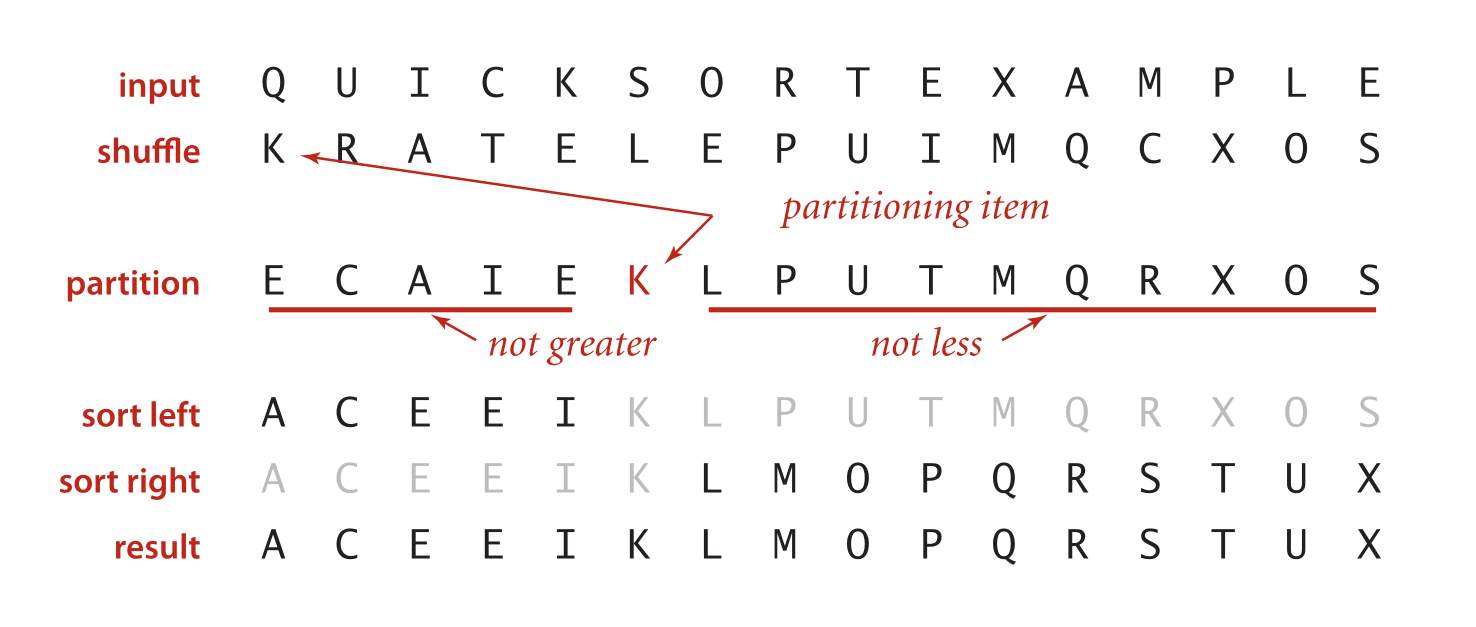
\includegraphics[width=\textwidth]{img/quicksort_overview.png}
    \caption{Fonte: \cite{sedgewick2014algorithms}}
  \end{figure}
\end{frame}

\begin{frame}[fragile]
  \frametitle{Tony Hoare}

  \begin{itemize}
    \item Inventou Quicksort para traduzir Russo para Inglês;
    \item Aprendeu Algol 60 (e recursão);
    \item Implementou Quicksort;
  \end{itemize}

  \begin{figure}
    \centering
    \begin{minipage}{.45\textwidth}
      \centering
      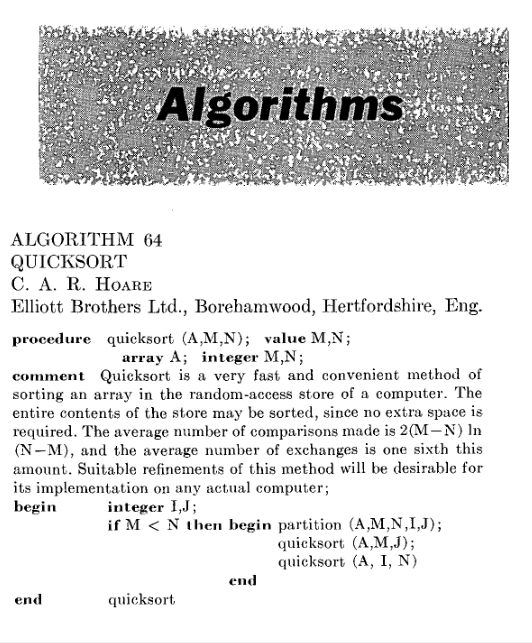
\includegraphics[width=0.8\textwidth]{img/paper_hoare.png}
      \caption{Communications of the ACM (Julho 1961)}
    \end{minipage}
    \begin{minipage}{.45\textwidth}
      \centering
      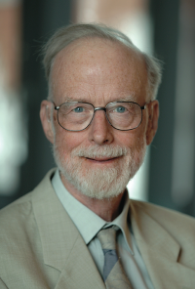
\includegraphics[width=0.5\textwidth]{img/hoare.png}
      \caption{Tony Hoare - 1980 Turing Award}
    \end{minipage}
  \end{figure}
\end{frame}


\begin{frame}[t]
  \frametitle{Tony Hoare}

  \begin{figure}
    \centering
    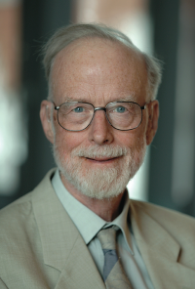
\includegraphics[width=0.2\textheight]{img/hoare.png}
    \caption{Tony Hoare - 1980 Turing Award}
  \end{figure}

  \only<1>{\begin{quotation}
    ``Existem duas formas para construir um software: uma delas é criá-lo tão simples de forma que, obviamente, não existam deficiências, e a outra é criá-lo tão complexo de forma que não existam deficiências óbvias. O primeiro modo é muito mais difícil.'' 
  \end{quotation}}
  \only<2>{\begin{quotation}
    ``Eu chamo de "meu erro de um bilhão de dólares". Foi a invenção do "Null reference" (para Algol) em 1965... Isso levou incontáveis erros, vulnerabilidades e crashs de sistemas, o que provavelmente causou bilhões de dólares em danos e dores nos últimos quarenta anos.'' 
  \end{quotation}}
\end{frame}

\begin{frame}[t]
  \frametitle{Bob Sedgewick}

  \begin{minipage}[t]{.7\textwidth}
    \begin{itemize}
      \item Refinou e populariou o quicksort;
      \item Analisou várias versões do algoritmo;
    \end{itemize}
  \end{minipage}
  \begin{minipage}[t]{.2\textwidth}
    \begin{figure}
      \centering
      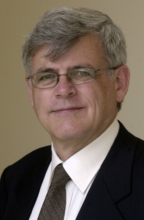
\includegraphics[width=0.5\textwidth]{img/sedgewick.png}
      \caption{Bob Sedgewick}
    \end{figure}
  \end{minipage}

  \begin{figure}
    \centering
    \begin{minipage}{.35\textwidth}
      \centering
      
\includegraphics[width=0.8\textwidth]{img/paper_sedgewick_1.png}
    \end{minipage}
    \begin{minipage}{.75\textheight}
      \centering
      
\includegraphics[width=0.9\textwidth]{img/paper_sedgewick_2.png}
    \end{minipage}
  \end{figure}
\end{frame}


\begin{frame}[t]
  \frametitle{Particionamento Simples}

  Repita até que \tcb{i} e \tcb{j} se cruzem:
  \begin{itemize}
    \item Varrer \tcb{i} da esquerda para a direita enquanto $a[i] < a[lo]$;
    \item Varrer \tcb{j} da esquerda para a direita enquanto $a[j] > a[lo]$;
    \item Troque $a[i]$ com $a[j]$.
  \end{itemize}

  \vspace{1cm}

  \multiinclude[<+->][format=png, graphics={width=\textwidth}]{img/partition/partition}
\end{frame}

\begin{frame}[fragile,c]{Implementação Particionamento Simples}
  \begin{minted}[frame=lines,framesep=2mm,baselinestretch=1,fontsize=\smaller,linenos]{c}
int partition(int * a, int lo, int hi)
{
  int i = lo, j = hi+1;
  while(1)
  {
    while(a[++i] < a[lo]) // Encontra item na esquerda para a troca
    if(i == hi) break;

    while(a[lo] < a[--j]) // Encontra item na direita para a troca
    if(j == lo) break;

    if(i >= j) break;     // Checa se ponteiros se cruzam
    swap(a, i, j);        // Troca
  }

  swap(a, lo, j);         // Troca com o pivo
  return(j);              // Retorna o índice do elemento na 
}                         // sua posição "ordenada"
  \end{minted}
\end{frame}

\begin{frame}
	\frametitle{Particionamento Simples}
  \begin{figure}[h]
  	\centering
  	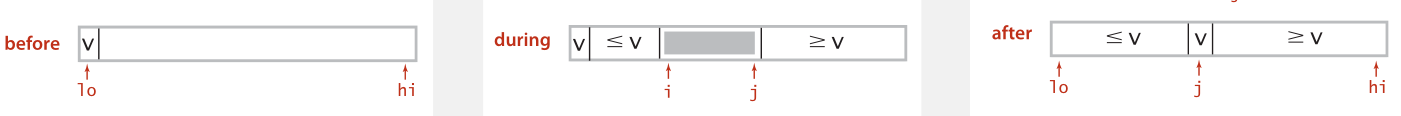
\includegraphics[width=\textwidth]{img/partition_steps.png}
  	\label{label}
  \end{figure}
\end{frame}

\begin{frame}[fragile,c]{Implementação Quicksort}
  \begin{minted}[frame=lines,framesep=2mm,baselinestretch=1,fontsize=\smaller,linenos]{c}
int partition(int * a, int lo, int hi);

void quicksort_(int * a, int lo, int hi)
{
  if(hi <= lo) return;
  int j = partition(a, lo, hi);
  quicksort_(a, lo, j-1);
  quicksort_(a, j+1, hi);
}

void quicksort(int * a, int n)
{
  shuffle(a,n);        // Veremos a seguir a importância do shuffle
  quicksort_(a,0,n-1);
}
  \end{minted}
\end{frame}

\begin{frame}
	\frametitle{Execução Quicksort}
  \begin{figure}[h]
  	\centering
  	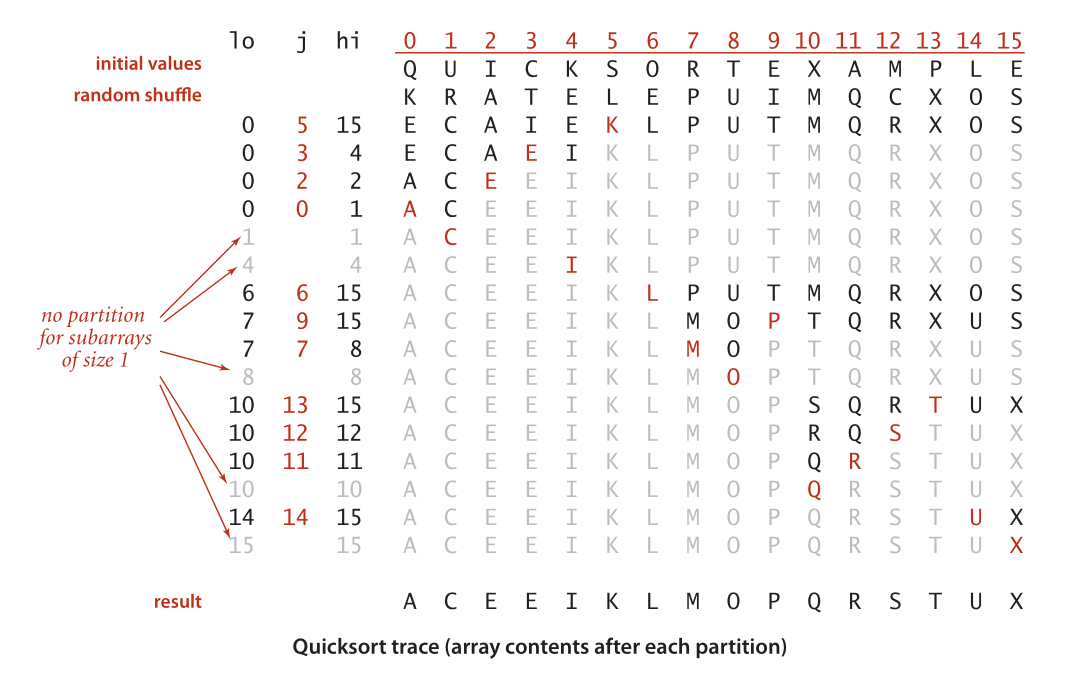
\includegraphics[width=\textwidth]{img/quicksort_trace.png}
  \end{figure}
\end{frame}

\begin{frame}
  \frametitle{Detalhes de implementação}

  \begin{description}
    \item[Particionamento \textit{in-place}] Utilizar um array adicional torna o particionamento mais fácil (e estável), mas não vale o custo;
    %\item[Término do laço] Determinar quando os ponteiros se cruzam é mais complicado do que parece;
    \item[Chaves iguais] Quando chaves repetidas estão presentes, é melhor parar a varredura em chaves iguais a do pivô;
  \end{description}

  \vspace{1cm}
      
  \begin{description}
    \item[Manter aleatoriedade] Shuffle é necessário para ``garantia'' de performance;
    \item[Alternativa equivalente] Escolher um pivô aleatório em cada subarray;
  \end{description}

\end{frame}

\begin{frame}[t]
  \frametitle{Análise empírica (1961)}

  Estimativas de desempenho:
  \begin{itemize}
    \item Implementação em Algol 60;
    \item Computador: National Elliott 405.
  \end{itemize}

  \begin{figure}
    \centering
    \begin{minipage}{.7\textwidth}
      \centering
      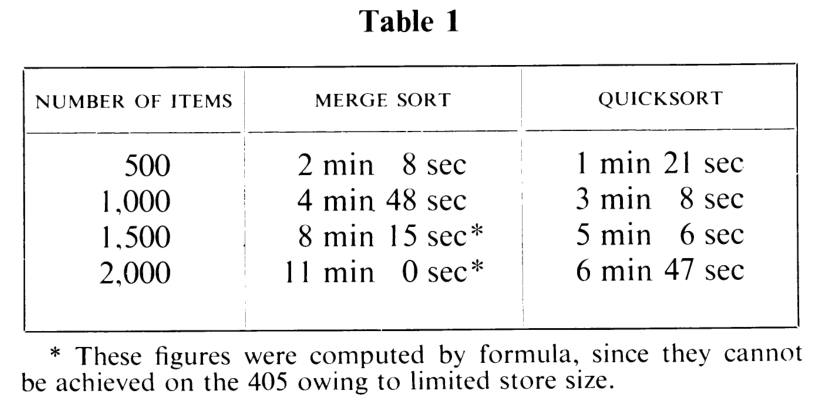
\includegraphics[width=0.95\textwidth]{img/empirico_algol.png}
      \caption{Ordenação de $n$ palavras de tamanho 6 com chaves de uma palavra.}
    \end{minipage}
    \begin{minipage}{.28\textwidth}
      \centering
      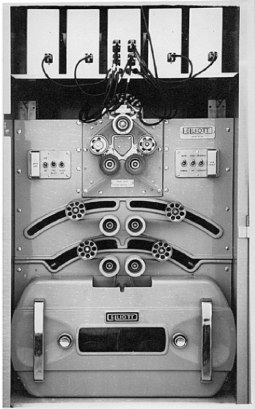
\includegraphics[width=0.8\textwidth]{img/elliott.png}
      \caption{Elliott 405 magnect disc (16k palavras)}
    \end{minipage}
  \end{figure}
\end{frame}

\begin{frame}[t]
  \frametitle{Análise empírica}

  Estimativas de desempenho:
  \begin{itemize}
    \item Computador doméstico executa $10^8$ comparações por segundo;
      \item Super computador executa $10^{12}$ comparações por segundo;
  \end{itemize}

  \begin{figure}
    \centering
    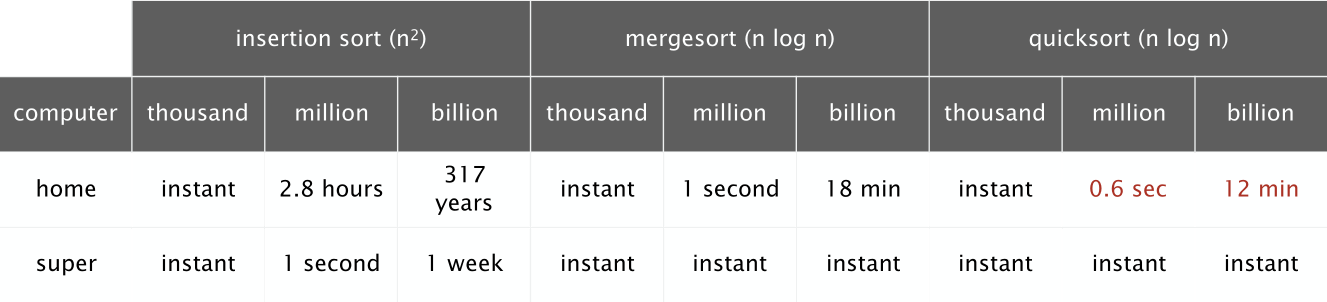
\includegraphics[width=0.95\textwidth]{img/empirico_atual.png}
  \end{figure}

  \begin{description}
    \item[Lição 1] Bons algoritmos são melhores do que super computadores.
    \item[Lição 2] Grandes algoritmos são melhores do que bons algoritmos. 
  \end{description}
\end{frame}

\begin{frame}[t]
  \frametitle{Análise Quicksort}

  \begin{description}
    \item[Melhor caso] Número de comparações é aprox. $n\log_{2}{n}$.
  \end{description}

  \begin{figure}
    \centering
    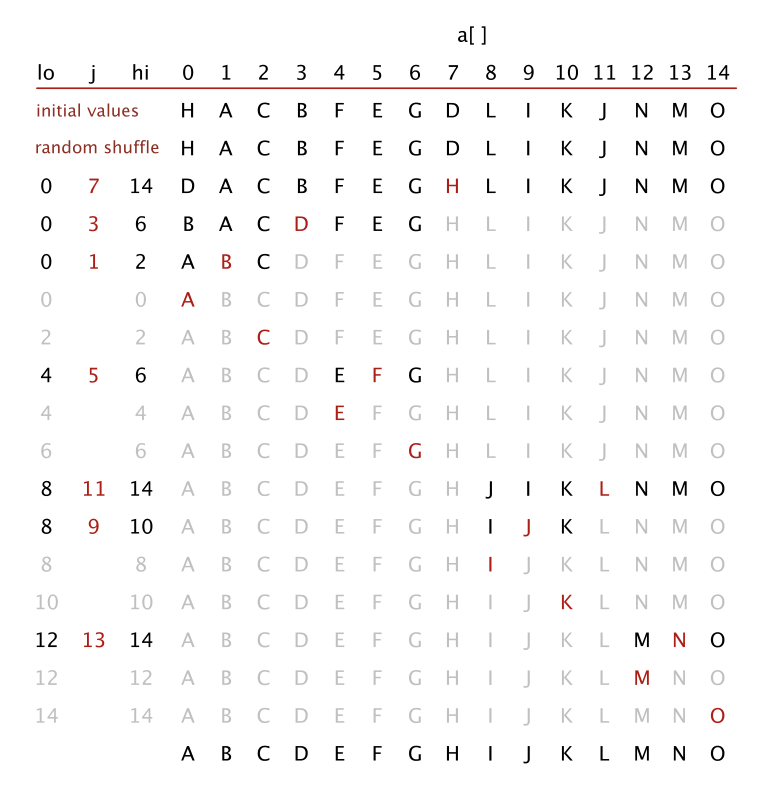
\includegraphics[width=0.7\textheight]{img/melhor_caso.png}
  \end{figure}

\end{frame}

\begin{frame}[t]
  \frametitle{Análise Quicksort}

  \begin{description}
    \item[Pior caso] Número de comparações é aprox. $\frac{1}{2}n^2$.
  \end{description}

  \begin{figure}
    \centering
    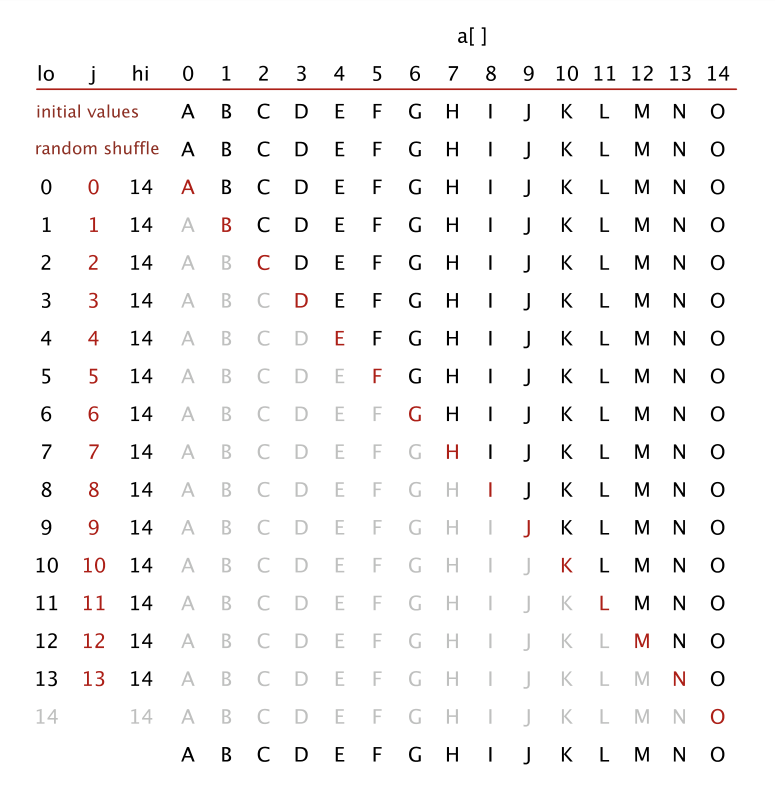
\includegraphics[width=0.7\textheight]{img/pior_caso.png}
  \end{figure}

\end{frame}

\begin{frame}[fragile]
  \frametitle{Resumo Análise Quicksort}

  Quicksort é um algoritmo probabilístico (\textit{randomized}, ou \textit{Las Vegas}):
  \begin{itemize}
    \item Corretude garantida;
    \item Tempo de execução depende do \textit{shuffle} aleatório;
  \end{itemize}

  \begin{description}
    \item[Caso médio] Número de comparações para um array de $n$ chaves \textbf{distintas} é $~ 1.39 \log_{2}{n}$ (e o número de trocas é $~\frac{1}{3}{n}\log_{2}{n}$):
  \end{description}

  \begin{itemize}
    \item 39\% mais comparações do que o Mergesort;
    \item Mais rápido do que o Mergesort na prática pois realiza menos movimentação de dados;
  \end{itemize}

  \begin{description}
    \item[Melhor caso] Número de comparações é $~ n \log_{2}{n}$;
    \item[Pior caso] Número de comparações é $~ \frac{1}{2} n^2$; \textcolor{gray}{Mas é mais provável que um raio caia no computador durante a execução}
  \end{description}

\end{frame}

\begin{frame}
  \frametitle{Propriedades Quicksort}

  Implementação apresentada (e a maioria delas) é:
  \begin{itemize}
    \item In-place; \only<2->{\textcolor{gray}{Particionamento utiliza espaço constante e altura da árvore de recursão é, provavelmente logarítmica}}
    \item Não estável; \only<3->{\textcolor{gray}{Contra-exemplo}}
  \end{itemize}

  \only<4>{
    \begin{figure}[h]
      \centering
      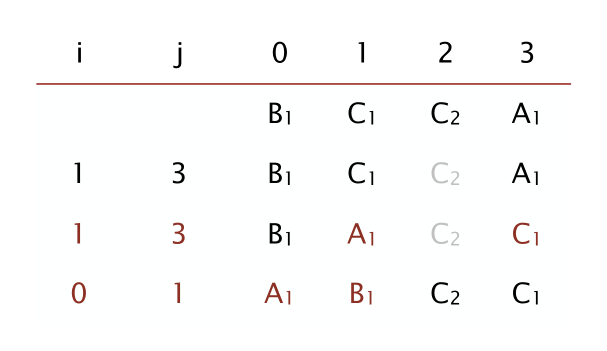
\includegraphics[width=0.5\textheight]{img/nao_estavel.png}
    \end{figure}
  }

  \only<1-3>{
  \vspace{3cm}
    Por quê?}
\end{frame}

\begin{frame}
  \frametitle{Insertion sort para pequenos subarrays}

  \begin{itemize}
    \item Até mesmo Quicksort possui mais overhead para pequenos arrays do que Insertion sort;
    \item Aplicar \textit{cutoff} (10 pode ser um bom número);
  \end{itemize}

\end{frame}

\begin{frame}
  \frametitle{Mediana para pivô}

  \begin{itemize}
    \item Melhor pivô? Mediana do array (divide a coleção exatamente ao meio);
    \item Utilizar a mediana exata o array (caro);
    \item Utilizar a mediana entre uma amostra qualquer (tamanho 3) do array (boa aproximação);
    \item Já evita o pior caso!
  \end{itemize}

\end{frame}

\begin{frame}
  \frametitle{Chaves iguais}

  \begin{minipage}{0.7\textwidth}
    \begin{itemize}
      \item Em aplicações práticas é comum que o conjunto de dados a ser ordenado possua algumas chaves iguais (elementos repetidos);
      \item Assim como no Mergesort, é possível tirar proveito de coleções desse tipo para melhorar o desempenho do Quicksort;
      \item Alias, a implementação vista não possui um bom desempenho para coleções com vários elementos repetidos. Consegue perceber porquê?

    \end{itemize}
  \end{minipage}
  \begin{minipage}{0.3\textwidth}
    \begin{figure}[h]
      \centering
      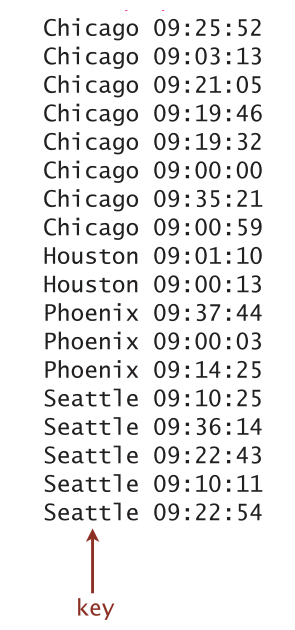
\includegraphics[width=0.8\textwidth]{img/chaves_repetidas.png}
    \end{figure}
  \end{minipage}

\end{frame}


\begin{frame}
  \frametitle{Chaves iguais}

  Nosso algoritmo de particionamento para a varredura quando encontra elementos iguais ao pivô:

  \begin{figure}[h]
    \centering
    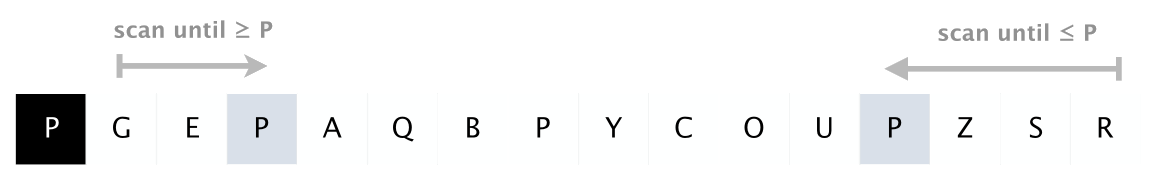
\includegraphics[width=0.8\textwidth]{img/stop_equal.png}
  \end{figure}
  
  Por que não continuar a varredura quando encontra elementos iguais ao pivô?

  \begin{figure}[h]
    \centering
    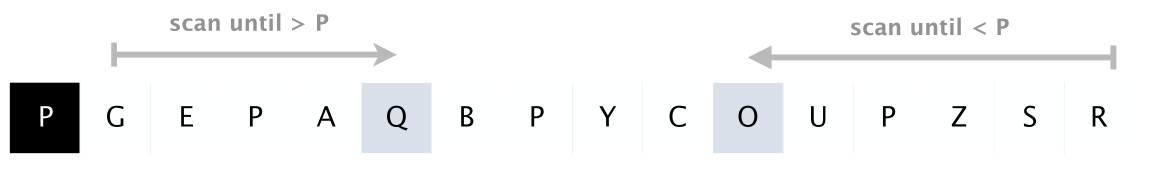
\includegraphics[width=0.8\textwidth]{img/non_stop_equal.png}
  \end{figure}

\end{frame}


\begin{frame}
  \frametitle{Chaves iguais: estratégias de particionamento}

  \begin{description}
    \item[Ruim] Não interromper varredura em chaves iguais ao pivô\\
                \textcolor{gray}{$\sim \frac{n^2}{2}$ comparações quando todos os elementos são iguais}
  \end{description}

  \begin{minipage}{0.5\textwidth}
    \centering
    \tiny{\vet{B, A, A , B, A, B, B, \tcr{B}, C, C, C}}
  \end{minipage}
  \begin{minipage}{0.5\textwidth}
    \centering
    \tiny{\vet{\tcr{A}, A, A , A, A, A,A, A, A, A, A}}
  \end{minipage}

  \begin{description}
    \item[Bom] Interromper varredura em chaves iguais ao pivô\\
                \textcolor{gray}{$\sim n \log_{2}{n}$ comparações quando todos os elementos são iguais}
  \end{description}

  \begin{minipage}{0.5\textwidth}
    \centering
    \tiny{\vet{B, A, A , B, A, \tcr{B}, C, C, B, C, B}}
  \end{minipage}
  \begin{minipage}{0.5\textwidth}
    \centering
    \tiny{\vet{A, A, A , A, A, \tcr{A},A, A, A, A, A}}
  \end{minipage}

  \begin{description}
    \item[Melhor] Colocar todas as chaves iguais ao pivô no lugar correto. Mas como?
                \textcolor{gray}{$\sim n$ comparações quando todos os elementos são iguais}
  \end{description}

  \begin{minipage}{0.5\textwidth}
    \centering
    \tiny{\vet{A, A, A , \tcr{B}, \tcr{B}, \tcr{B}, \tcr{B}, \tcr{B}, C, C, C}}
  \end{minipage}
  \begin{minipage}{0.5\textwidth}
    \centering
    \tiny{\vet{\tcr{A},\tcr{A},\tcr{A},\tcr{A},\tcr{A},\tcr{A},\tcr{A},\tcr{A},\tcr{A},\tcr{A},\tcr{A}}}
  \end{minipage}

\end{frame}

\begin{frame}
  \frametitle{Problema da Bandeira da Holanda}

  \begin{description}
    \item[Problema] \textcolor{gray}{[Edsger Dijkstra]} Dado um array de N posições e cada posição contendo uma cor (vermelhor, azul ou branco), ordene o array segundo as cores da bandeira da Holanda.
  \end{description}
  
  \begin{figure}[h]
    \centering
    
\includegraphics[width=0.8\textwidth]{img/dutch_national_flag_problem.png}
  \end{figure}

  Operações permitidas:
  \begin{itemize}
    \item \textit{swap(i,j)}: trocar as cores das posições $i$ e $j$;
    \item \textit{color(i)}: retorna a cor da posição $i$;
  \end{itemize}
  
  Requisitos da solução:
  \begin{itemize}
    \item Exatamente $n$ chamadas para \textit{color()};
    \item No máximo $n$ chamadas para \textit{swap()};
    \item Espaço extra constante.
  \end{itemize}

\end{frame}

\begin{frame}
  \frametitle{Partição em 3 partes}

  Partição em três partes, tal que:
  \begin{itemize}
    \item Valores entre $lt$ e $gt$ são iguais ao pivô;
    \item Nenhum valor maior à esquerda de $lt$;
    \item Nenhum valor menor à direita de $gt$;
  \end{itemize}
  
  \begin{figure}[h]
    \centering
    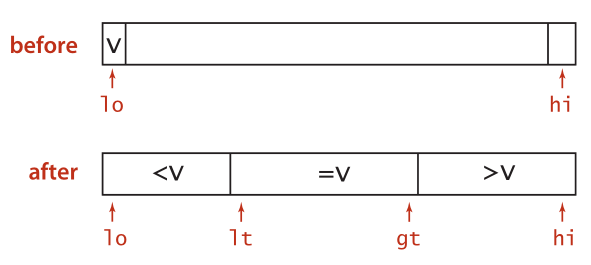
\includegraphics[width=0.5\textwidth]{img/3_way_partitioning.png}
  \end{figure}

  Problema da bandeira da Holanda \textcolor{gray}{[Edsger Dijkstra]}:
  \begin{itemize}
    \item Entendimento até metade de 1990: não vale a pena resolver;
    \item Atualmente, Partição em 3 partes foi incorporada à biblioteca C (qsort()) e ao Java.
  \end{itemize}

\end{frame}

\begin{frame}[t]
  \frametitle{Dijkstra Particionamento em 3 partes}

  \begin{itemize}
    \item Seja $v$ o pivô, na posição $a[lo]$;
    \item Varrer da esquerda para a direita com a variável $i$:
      \begin{itemize}
        \item $(a[i] < v)$: troca $a[lt]$ com $a[i]$; incrementa ambos $lt$ e $i$;
        \item $(a[i] > v)$: troca $a[gt]$ com $a[i]$; decrementa $gt$;
        \item $(a[i] == v)$: incrementa $i$;
      \end{itemize}
  \end{itemize}

  \vspace{2cm}

  \multiinclude[<+->][format=png, graphics={width=\textwidth}]{img/3_way_partition/3_way_partition}
\end{frame}

\begin{frame}[c]
  \frametitle{Implementação Particionamento em 3 partes}

  \center ???
\end{frame}

\begin{frame}
	\frametitle{Execução 3-way Quicksort}
  \begin{figure}[h]
  	\centering
  	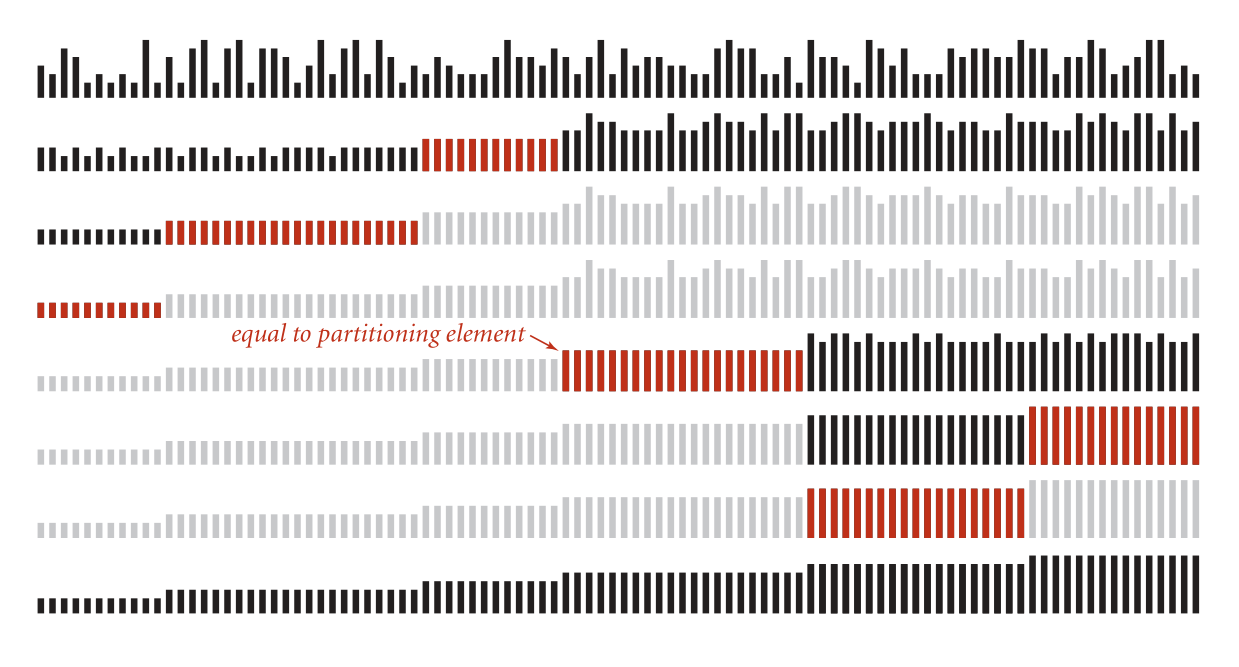
\includegraphics[width=\textwidth]{img/3_way_quicksort_trace.png}
  \end{figure}

  3-way Quicksort reduz o tempo de execução de Linearítmico para linear em uma grande classe de aplicações.
\end{frame}

\begin{frame}
	\frametitle{Resumo Ordenação}
  \begin{figure}[h]
  	\centering
  	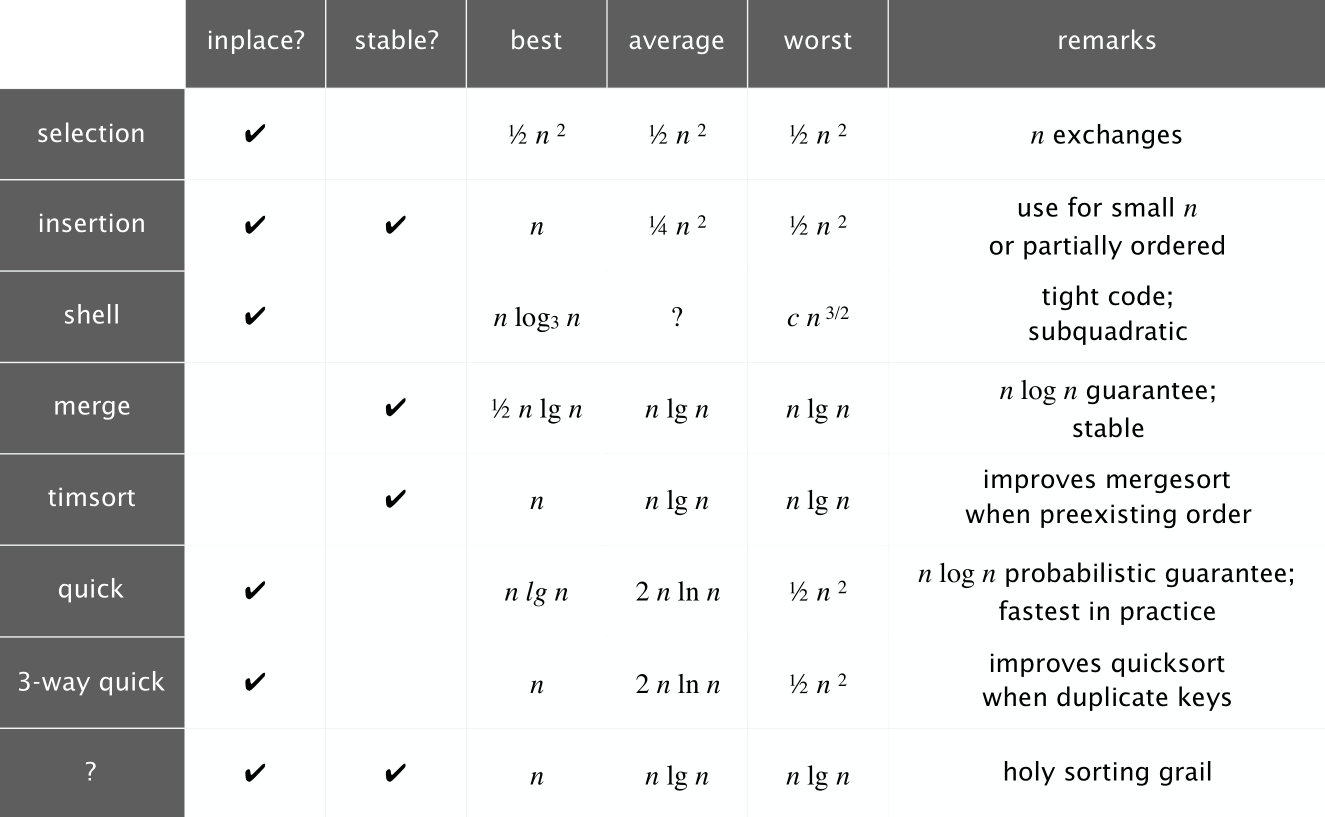
\includegraphics[width=\textwidth]{img/sorting_sumary.png}
  \end{figure}
\end{frame}


% ==========================================
% \begin{frame}[fragile,c]{Implementação Recursiva Fatorial}
%	\begin{minted}[frame=lines,framesep=2mm,baselinestretch=1.2,fontsize=\normalsize,linenos]{c}
%	\end{minted}
% \end{frame}
% ==========================================

% ==========================================
% \begin{frame}
% 	\frametitle{Título}
% 	\begin{itemize}
% 		\item Item bla bla bla
% 	\end{itemize}
%	  \begin{block}{Título de bloco}
%		 	Conteúdo do bloco
%   \end{block}
% \end{frame}
% ==========================================

% ==========================================
% Exemplo de frame com figura
% \begin{frame}
% 	\frametitle{Título}
%	  \begin{figure}[h]
%	  	\centering
%	  	\includegraphics[width=10cm]{paht.png}
%			\caption{Bla bla bla ...}
%	  	\label{label}
%	  \end{figure}
% \end{frame}
% ==========================================

% ==========================================
% Exemplo de frame com algoritmo
% \begin{frame}[fragile]
% 	\frametitle{Título}
% 	\begin{lstlisting}[language=C]
% 		#include <stdio.h>
%
% 		int main()
% 		{
% 		  int a[5];
%
% 		  a[0] = 30;
% 		  a[1] = 25;
% 		  a[2] = 5;
% 		  a[3] = 100;
% 		  a[4] = 1;
%
% 		  printf("%d\n",a[1]);
% 		}
% 	\end{lstlisting}
% \end{frame}
% ==========================================

% ==========================================
% Frame para referências
\begin{frame}[allowframebreaks]
  \frametitle{Referências utilizadas na apresentação}
  \bibliography{referencias}
\end{frame}
% ==========================================

\end{document}
